\section{Svahy}\index{svah}
Svah -- ukloněná část zemského povrchu je nejrozšířenějším a také nejdynamičtějším prvkem reliéfu krajiny. Svahy zabírají přibližně $90 \%$ povrchu souše. Většina svahů (cca $60 \%$) má sklon do \SI{10}{\degree}. 

V základu můžeme rozlišovat dva typy svahů.  A to podle toho, zda jsou pokryté sedimenty či půdou (\textit{soil-mantled hillslopes}). Tyto svahy jsou charakteristické svým hladkým průběhem s jen občasnými výchozy podloží. Druhým typem jsou svahy tvořené jen skalním podložím, neboli strukturní svahy (\textit{bedrock hillslopes}). Takovéto svahy jsou typické rozeklaným povrchem.


\subsection{Části svahu}
Svah lze rozčlenit do několika částí (jednotek, segmentů). Nejjednodušší rozdělení je do tří jednotek (Obr. \ref{fig:segmenty_svahu}. V horní části je konvexní jednotka, kde se sklon svahu s narůstající vzdáleností zvětšuje. Následuje lineární svah (sklon se nemění). Spodní část svahu má konkávní tvar, což znamená, že se sklon zmenšuje. V některých případech prostřední část svahu chybí a má konvexně-konkávní průběh \parencite{whiteConvexConcaveLandslopesGeometrical1966}. Přechod mezi jednotlivými segmenty může být pozvolný ale i ostrý.

\begin{figure}[h]
	\centering
	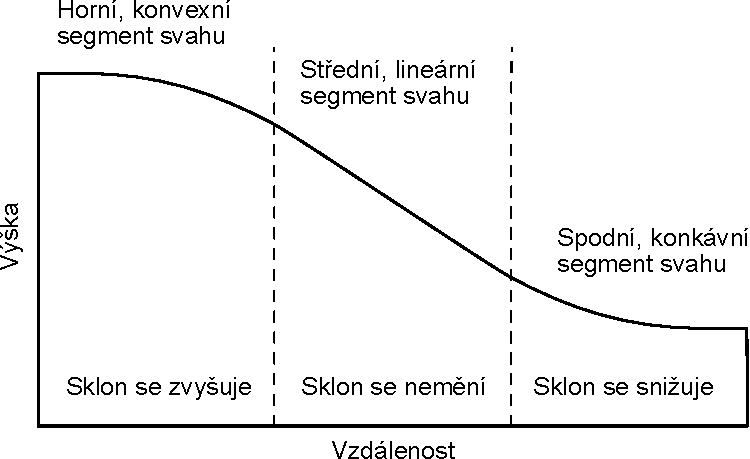
\includegraphics[width=1\linewidth]{obrazky/slope/segmenty_svahu}
	\caption{Tři základní segmenty svahu.}
	\label{fig:segmenty_svahu}
\end{figure}


Pojmenováním jednotlivých částí svahu se zabývala celá řada autorů. \textcite{dalrympleHypotheticalNineUnit1968} rozdělili svah do osmi částí:
\begin{enumerate}
	\item rozvodní část svahu o sklonu \SIrange{0}{1}{\degree}
	\item konvexní infiltrační část svahu se sklonem \SIrange{2}{4}{\degree}
	\item konvexní část svahu s plíživým pohybem materiálu 
	\item srub se sklonem minimálně \SI{45}{\degree}, zpravidla ale se sklonem přes \SI{65}{\degree}
	\item konkávní erozně-denudační část se sklonem \SIrange{26}{35}{\degree} kde probíhá transport materiálu
	\item konkávní akumulační část svahu
	\item fluviální část svahu v dosahu říční činnosti
	\item samotné říční koryto
\end{enumerate}

\subsection{Síly působící na svah}
Každá část svahu je pod vlivem gravitace. Ta vyvolává tíhové napětí. Pro zjednodušení si představte objekt který je na nakloněné rovině -- svahu. Tento objekt svou tíhou působí svisle na svah a vyvolává tíhové napětí. To můžeme rozložit do dvou složek. \emph{Normálová} složka resp. \emph{normálové napětí} působí kolmo na rovinu svahu. Po svahu dolů působí \emph{smykové napětí}. Smykové a normálové napětí vypočítáme podle rovnic:

\begin{align}
\text{Smykové napětí: }	\tau = \rho_{s}gz\sin{\theta}\\
\text{Normálové napětí: }	\sigma = \rho_{s}gz\cos{\theta}
\end{align}

Velikost smykového a normálového napětí je závislá na velikosti sklonu ($\theta$) svahu. S rostoucím sklonem narůstá smykové napětí a normálové klesá a naopak. Na horizontálním povrchu je smykové nulové, normálové napětí se rovná tíhovému. U kolmé stěny je naopak nulové normálové napětí a smykové se rovná tíhovému napětí.

\begin{figure}[h]
	\centering
	\includegraphics[width=1\linewidth]{obrazky/slope/svah_napeti}
	\caption{A: Rozklad tíhového napětí (síly) na normálové napětí ($\sigma$) a smykové napětí ($\tau$) v závislosti na sklonu svahu ($\beta$). B: ukázka rozložení sil na svahu (upraveno podle \textcite{selbyHillslopeMaterialsProcesses1993})}
	\label{fig:svahnapeti}
\end{figure}

\subsection{Koncept stability svahu}
Koncept stability svahu souvisí s působením výše uvedených sil (napětí) ve svahu. Ve své podstatě se jedná o poměr mezi silami, které drží materiál svahu v původní poloze a silami, které se snaží jej uvést do pohybu. Stabilita svahu tedy lze vyjádřit rovnicí:

\begin{equation}
\text{stabilita svahu} = \frac{\text{síly držící svah}}{\text{mobilizační síly}}	
\end{equation}

Poměr těchto sil se označuje jako faktor bezpečnosti (\textit{factor of safety}, FS) a ten vypočítáme jako podíl pevnosti ve smyku ($S$) a smykového napětí ($\tau$):

\begin{equation}
	\text{FS} = \frac{s}{\tau}	
\end{equation}

Svah je stabilní pokud je faktor bezpečnosti větší než jedna. Zpravidla se vyčleňují tři \enquote{pásma stability}:

\begin{itemize}
	\item FS $>1,3$ jedná se o stabilní svah
	\item FS z intervalu $(1;1,3>$ se jedná o podmínečně stabilní svah
	\item FS $=<1$ se jedná se o nestabilní svah
\end{itemize}

Pevnost ve smyku (\textit{shear strength}, S) lze vypočítat podle Coulomb-Terzagiho rovnice následovně:

\begin{equation}
	S = c+\sigma^{\prime}\tan{\phi}
\end{equation}

\emph{Koheze materiálu} ($c$) nebo také soudržnost materiálu je veličina, která udává jak jednotlivé částice materiálu drží pospolu. Je nezávislá na vnějších tlacích a je dána zejména chemickými vazbami a adhezí.

\emph{Úhel vnitřního tření materiálu} je závislý na velikosti částic, jejich tvarem a rozmítění.

\emph{Normálové napětí} zvyšuje úhel vnitřního tření. Jelikož proti normálovému napětí působí tlak vody v pórech (tzv. pórové tlaky) snižuje se o jejich hodnotu velikost normálového napětí. Hovoříme potom o \emph{efektivním normálovém napětí} ($\sigma^{\prime}$).

Stabilita svahu je stav, který se mění v čase v závislosti na celé řadě podmínek. Může se zvyšovat, ale i snižovat. 

Tabulka \ref{tab:stabilita_faktory} obsahuje příklady různých příčin sesuvů a jiných svahových pohybů. Tyto příčiny můžeme rozdělit do tří skupin:
\begin{enumerate}
	\item Predispozice
	\item Přípravné faktory
	\item Spouštěcí faktory
\end{enumerate}

\emph{Predispozice} jsou vlastnosti hornin, kterými je svah budován (např. koheze, pevnost materiálu), přítomnost a orientace tektonických struktur (pukliny), sklon, výška svahu a podobně. \emph{Přípravné faktory} způsobují postupné snižování stability svahu. Například zvětráváním horniny může docházet ke snižování koheze, rozpouštění tmele, který drží jednotlivé klasty. Akumulací sedimentů v horní části svahu dochází k zatěžování svahu (roste ve svahu smykové napětí). \emph{Spouštěcí faktory} jsou ty, které svah uvedou do pohybu. Způsobí tedy to, že se faktor bezpečnosti sníží na jedna a méně. Spouštěcím faktorem může být například zemětřesení, které ve svahu vyvolává přechodné napětí. Významným spouštěčem jsou intenzivní srážky, které způsobují zvýšení pórových tlaků (a tedy snížení normálového napětí).

\begin{figure}[h]
	\centering
	\includegraphics[width=1\linewidth]{obrazky/slope/stability_diagram}
	\caption{Faktory ovlivňující stabilitu svahu. V případě destabilizace svahu pak nastupují faktory, podporující nestabilitu svahu (upraveno podle \textcite{gladeLandslideGeomorphologyChanging2010})}
	\label{fig:stability_diagram}
\end{figure}

\begin{figure*}[h]
	\centering
	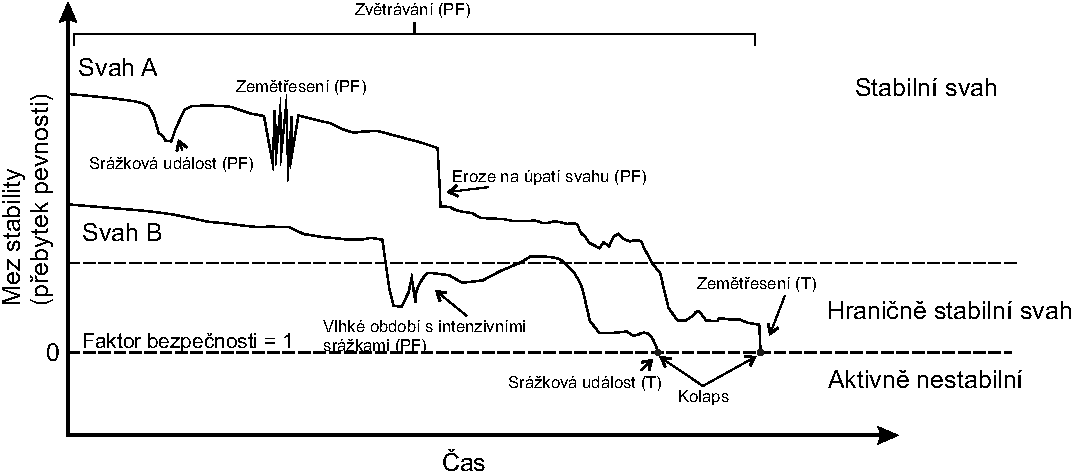
\includegraphics[width=1\linewidth]{obrazky/slope/time_stability}
	\caption{Vývoj stability dvou hypotetických svahů. Přípravné faktory (PF) postupně nebo nárazově snižují stabilitu svahu (snižují pevnost ve smyku). Spouštěcí faktory (triggery -- T) jsou ty, které sníží pevnost ve smyku tak, že faktor bezpečnosti $ \leq 1$ (upraveno podle \textcite{popescuSuggestedMethodReporting1994} a \textcite{mccollLandslideCausesTriggers2015})}
	\label{fig:timestability}
\end{figure*}

%\todo[inline]{Glade Crozier obrázek faktory}
%\todo[inline]{McColl svahy vývoj}
\begin{table*}
	\small
	\begin{tabularx}{\textwidth}{@{}XXXX@{}}
		\toprule
		\multicolumn{4}{@{} p{\textwidth} @{}}{\textbf{Predispozice}} \\
		\midrule
		\multicolumn{4}{@{} p{\textwidth} @{}}{Plastický, měkký materiál} \\
		\multicolumn{4}{@{} p{\textwidth} @{}}{Sypký materiál} \\
		\multicolumn{4}{@{} p{\textwidth} @{}}{Navětralý materiál} \\
		\multicolumn{4}{@{} p{\textwidth} @{}}{Tektonicky porušený materiál} \\
		\multicolumn{4}{@{} p{\textwidth} @{}}{Příhodně orientované diskontinuity (např. vrstevní plochy, pukliny, zlomy)}\\
		\multicolumn{4}{@{} p{\textwidth} @{}}{Kontrast mezi propustností hornin} \\
		\multicolumn{4}{@{} p{\textwidth} @{}}{Kontrastní pevnost hornin (pevné horniny v nadloží plastických např. pískovce na jílovcích)}\\ 
		\midrule \midrule
		& & \textbf{Proces} & \\ 
		\midrule
		\textbf{\textbf{Přípravné faktory}} & \textbf{Geomorfologický} & \textbf{Fyzikální} & \textbf{Antropogenní} \\ 
		\midrule
		Nárůst výšky svahu nebo sklonu  & Tektonické pochody, vulkanismus, výzdvih po odlednění &  & Výkopy ve svahu, násypy \\
		& Fluviální, marinní nebo ledovcová eroze &  &  \\
		Ztráta opory & Ústup ledovce &  & Odtěžení paty svahu \\
		Odkrytí potenciálních smykových ploch & Eroze &  & Výkopy ve svahu \\
		Snížení pevnosti horniny & Sufoze, rozpouštění & Zvětrávání & Hloubení tunelů, dolů; odlesnění\\ 
		& Zvětrávání & Únava materiálu &  \\
		Zatěžování svahu & Postupná akumulace sedimentů  &  &Stavba, ukládání materiálu -- výsypky  \\
		Dlouhodobé zvyšování hladiny podzemní vody & Klimatické změny &  & Infiltrace srážkových vod, prasklé potrubí  \\
		&  &  & Zavlažování \\
		&  &  & Odstranění vegetace \\ 
		\midrule \midrule
		\textbf{Spouštěče} & \textbf{Geomorfologické} & \textbf{Fyzikální} & \textbf{Antropogenní} \\ 
		\midrule
		Rychlý nárůst pórových tlaků  & Rychlé zatížení sedimenty z Undrained loading from rapid emplacement of sediment & Srážky & Zatížení rychlým uložením navážky  \\
		&  &  Tání sněhu/ledu &  \\
		Rychlý pokles hladiny podzemní vody & Protržení přírodních hrází &  & Snižování hladiny v nádržích \\
		Přechodná napětí&  & Zemětřesení& Vibrace strojů \\
		&  & Vítr &  \\
		Snížení pevnosti&  & Degradace permafrostu &  \\
		&  & Zvětrávání &  \\
		&  & Únava materiálu &  \\
		Zatěžování svahu & Jiné sesuvy & Srážky & Stavby \\
		\bottomrule
	\end{tabularx}
		\caption{Příklady příčin sesuvů \parencite[podle][]{mccollLandslideCausesTriggers2015}}
		\label{tab:stabilita_faktory}
	
\end{table*}

\section{Gravitační svahové pochody}

\subsection{Světová klasifikace svahových pohybů}
Gravitační svahové pohyby jsou způsobeny přímým působením gravitace. Dalo by se říct, že \enquote{klasickou} a celosvětově zaužívanou klasifikací svahových pohybů je klasifikace \textcite{crudenLandslideTypesProcesses1996} s poslední úpravou od Hungra \parencite*{hungrVarnesClassificationLandslide2014}. Tato klasifikace je založena na třech kritériích:
\begin{itemize}
	\item rychlost pohybu
	\item mechanismus pohybu
	\item typ horniny (skalní hornina/zemina)
\end{itemize}

Svahové pohyby rozdělují do následujících šesti skupin:
\begin{itemize}
	\item Řícení (\textit{fall})
	\item Odklánění (\textit{topple})
	\item Sesouvání (\textit{slide})
	\item Boční rozšiřování (\textit{spread})
	\item Tečení (\textit{flow})
	\item Svahové deformace (\textit{slope deformation})
\end{itemize}

\begin{figure*}
	\centering
	\includegraphics[width=1\linewidth]{obrazky/slope/landslide_type}
	\caption{Typy gravitačních svahových pohybů (Upraveno podle USGS)}
	\label{fig:landslidetype}
\end{figure*}


%\begin{table*}[]
%	\begin{tabular}{@{}lll@{}}
%		\toprule
%		Typ pohybu & Skalní horniny                       & Zeminy                            \\ \midrule
%		Řícení             & 1. Rock/ice fall           & 2. Boulder/debris/silt falla    \\ \midrule
%		\multirow{2}{*}{Odsedání/toppling}            & 3. Blokové odsedání          & 5. Odesdání štěrku/písku/siltu        \\ 
%		& 4. Flexurní odsedání    &                                 \\ \midrule
%		\multirow{5}{*}{Sesouvání}             & 6. Skalní rotační sesuv       & 11. Clay/silt rotational slide     \\
%		& 7. Rock planar slidea      & 12. Clay/silt planar slide      \\
%		& 8. Rock wedge slidea       & 13. Gravel/sand/debris slidea   \\ \midrule
%		& 9. Rock compound slide     & 14. Clay/silt compound slide    \\
%		& 10. Rock irregular slidea  &                                 \\ \midrule
%		\multirow{2}{*}{Spread}            & 15. Rock slope spread          & 16. Sand/silt liquefaction spreada \\
%		& 17. Sensitive clay spreada &                                 \\ \midrule
%		\multirow{9}{*}{Flow}              & 18. Rock/ice avalanchea        & 19. Sand/silt/debris dry flow      \\
%		&                            & 20. Sand/silt/debris flowslidea \\
%		&                            & 21. Sensitive clay flowslidea   \\
%		&                            & 22. Debris flowa                \\
%		&                            & 23. Mud flowa                   \\
%		&                            & 24. Debris flood                \\
%		&                            & 25. Debris avalanchea           \\
%		&                            & 26. Earthflow                   \\
%		&                            & 27. Peat flow                   \\ \midrule
%		\multirow{3}{*}{Slope deformation} & 28. Mountain slope deformation & 30. Soil slope deformation         \\
%		& 29. Rock slope deformation & 31. Soil creep                  \\
%		&                            & 32. Solifluction                \\ 
%		\bottomrule
%	\end{tabular}
%	\caption{HUngr varnes klasifikace}
%	\label{tab:sesuvy_Hungr}
%\end{table*}

\subsubsection{Řícení}
\emph{Řícení} (\textit{fall}) je nejrychlejším gravitačním procesem, kdy rychlost pohybu činí řádově \si{\metre\per\second}. K řícení dochází na strmých svazích ($>\SI{45}{\degree}$). Pohyb hmoty je alespoň v části trajektorie realizován volným pádem a následně se horninové fragmenty kutálejí či poskakují. Řícení můžeme rozlišit podle materiálu, který se účastní pohybu na: skalní řícení, suťové řícení a řícení v zeminách (spraši).

Řícení může nabývat celé řady podob. \emph{Sesypávání} probíhá nejčastěji v zeminách. Dále může docházet k \emph{odpadávání úlomků} ze skalních výchozů. Na úpatí skalní stěny se tvoří osypy (\textit{talus}). \emph{Odvalové řícení} je způsobeno odkláněním bloku (viz níže), kdy po překročení kritické meze dojde k jeho kolapsu. \emph{Planární řícení} zahrnuje podobně jako odvalové řícení větší masu horniny. V iniciální fázi dochází k sesouvání horniny podél planární smykové plochy a až následně dojde k pohybu volným pádem a tedy řícení. Jedná se často o velké katastrofické události.

\subsubsection{Odklánění}
\emph{Odklánění} nebo také \emph{odsedání} (\textit{toppling}) je proces, kdy dochází k pohybu horninového bloku kolem horizontální osy. V podstatě jde překlápění bloku ze svahu dolů. Jedná se o pomalé pohyby (\si{\milli\metre\per\rok}). Avšak ve finální fázi může dojít až ke katastrofickému zrychlení pohybu -- zřícení (\si{\metre\per\second}).

\textcite{goodmanTopplingRockSlopes1976} rozlišují dva základní druhy odklánění. Prvním typem je blokové odklánění. Jedná se o uklánění velkých bloků hornin. Predispozicí jsou strmě do svahu zapadající diskontinuity, které od sebe oddělují jednotlivé horninové bloky a případně doplněné o mírně ukloněné diskontinuity tvořící bázi bloků. Druhý typ je ohybové odklánění (\textit{flexural toppling}). K této deformaci může docházet na strmých svazích, které jsou budované horninami se strmě zapadajícími diskontinuitami s velmi malým rozestupem. K odklánění může docházet i v zeminách např. na březích vodních toků.

\subsubsection{Sesouvání}
\emph{Sesouvání} (\textit{slide}) je relativně rychlý, klouzavý pohyb horninové hmoty na svahu podél jedné nebo více \emph{smykových ploch}. Rychlost je variabilní, může se pohybovat v řádu \si{\milli\metre\per\rok}--\si{\metre\per\second}. Rychlost pohybu uvolněné hmoty se směrem do hloubky nemění.

\emph{Sesouvání je proces}, jehož výsledný tvar je \emph{sesuv}.

Sesuv má tři základní části: 
\begin{itemize}
	\item Odlučná oblast (výchoz smykové plochy)
	\item Transportní zóna
	\item Akumulační zóna
\end{itemize}

Smyková plocha je plocha, podél které došlo k sesouvání. Sesouvání může probíhat i po více smykových plochách. Podle tvaru smykové plochy můžeme sesuvy rozlišit na dva základní typy: rotační a translační sesuvy.

\emph{Rotační sesuv} (\textit{rotational slide} nebo \textit{slump}, obr. \ref{fig:rotacni}) má smykovou plochu zakřivenou, válcovou. Na tvar smykové plochy nemají vliv geologické struktury (pukliny, vrstevní plochy). Z důvodu zakřivení smykové plochy dochází k naklonění povrchu sesunutých bloků proti svahu. Rotační sesuvy jsou typické pro homogenní materiály, kohezivní zeminy a měkké horniny, které mají v nadloží často vrstvu pevných hornin. Jelikož je pohyb podél zakřivené smykové plochy samostabilizační, jsou rotační sesuvy zpravidla pomalejší.

\begin{figure}[h]
	\centering
	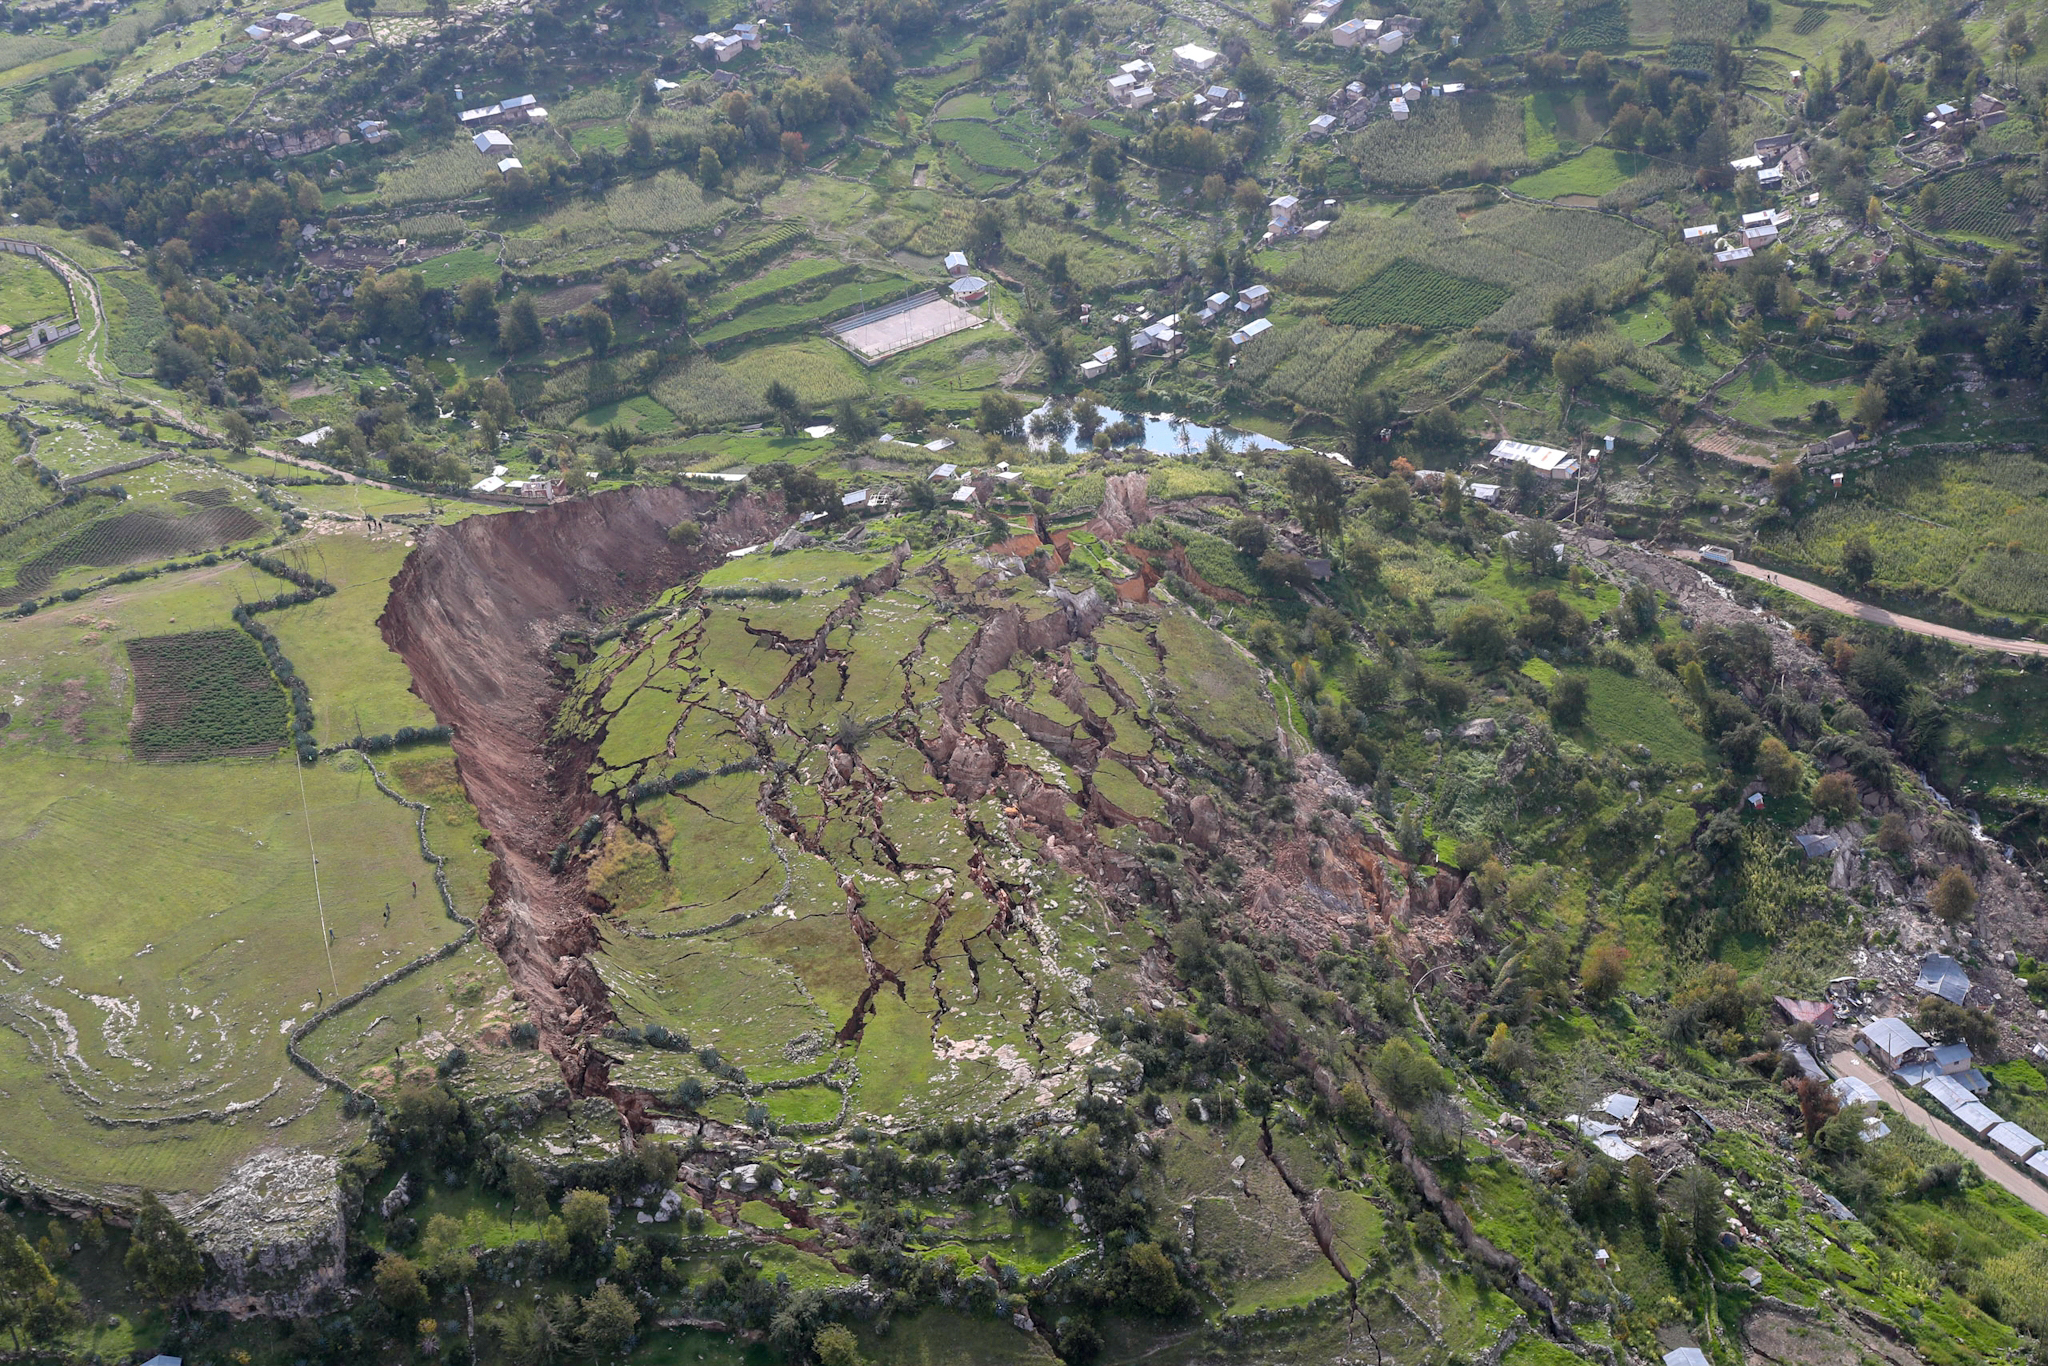
\includegraphics[width=1\linewidth]{obrazky/slope/rotacni}
	\caption{Rotační sesuv poblíž Cusca, Peru  roku 2018 (autor: Ministerio de Defensa del Perú - \url{https://www.flickr.com/photos/ministeriodedefensaperu/39935939755/in/dateposted/}, CC BY 2.0}
	\label{fig:rotacni}
\end{figure}


\emph{Translační} nebo také \emph{planární sesuvy} mají smykovou plochu rovnou. Ta je většinou predisponovaná nějakou nespojitostí v hornině. Může se jednat například o vrstevní plochy, pukliny, plochy foliace apod. Translační sesuvy ale mohou vznikat i na rozhraní sediment -- skalní podloží. Pokud se horninová masa pohybuje jako jeden celek po jedné smykové ploše, označujeme to jako \emph{blokový sesuv}. Specifickým typem translačních sesuvů jsou tzv. \textit{wedge slides} -- klínové sesuvy. Smyková plocha je tvořená zpravidla dvěma strukturami (např. puklinami), které oddělují nestabilní blok od zbytku skalního masivu. Na rozdíl od rotačních sesuvů nejsou translační sesuvy samostabilizační, tudíž se jedná zpravidla o velice rychlé události. Mělké planární sesuvy (vzniklé ve zvětralinách) vznikají často po intenzívních deštích. 

Některé sesuvy mohou mít složenou smykovou plochu. Běžný typ \emph{sesuvu podél složené smykové plochy} má v horní části zakřivenou smykovou plochu přecházející pak v planární níže po svahu.
\begin{figure*}
	\centering
	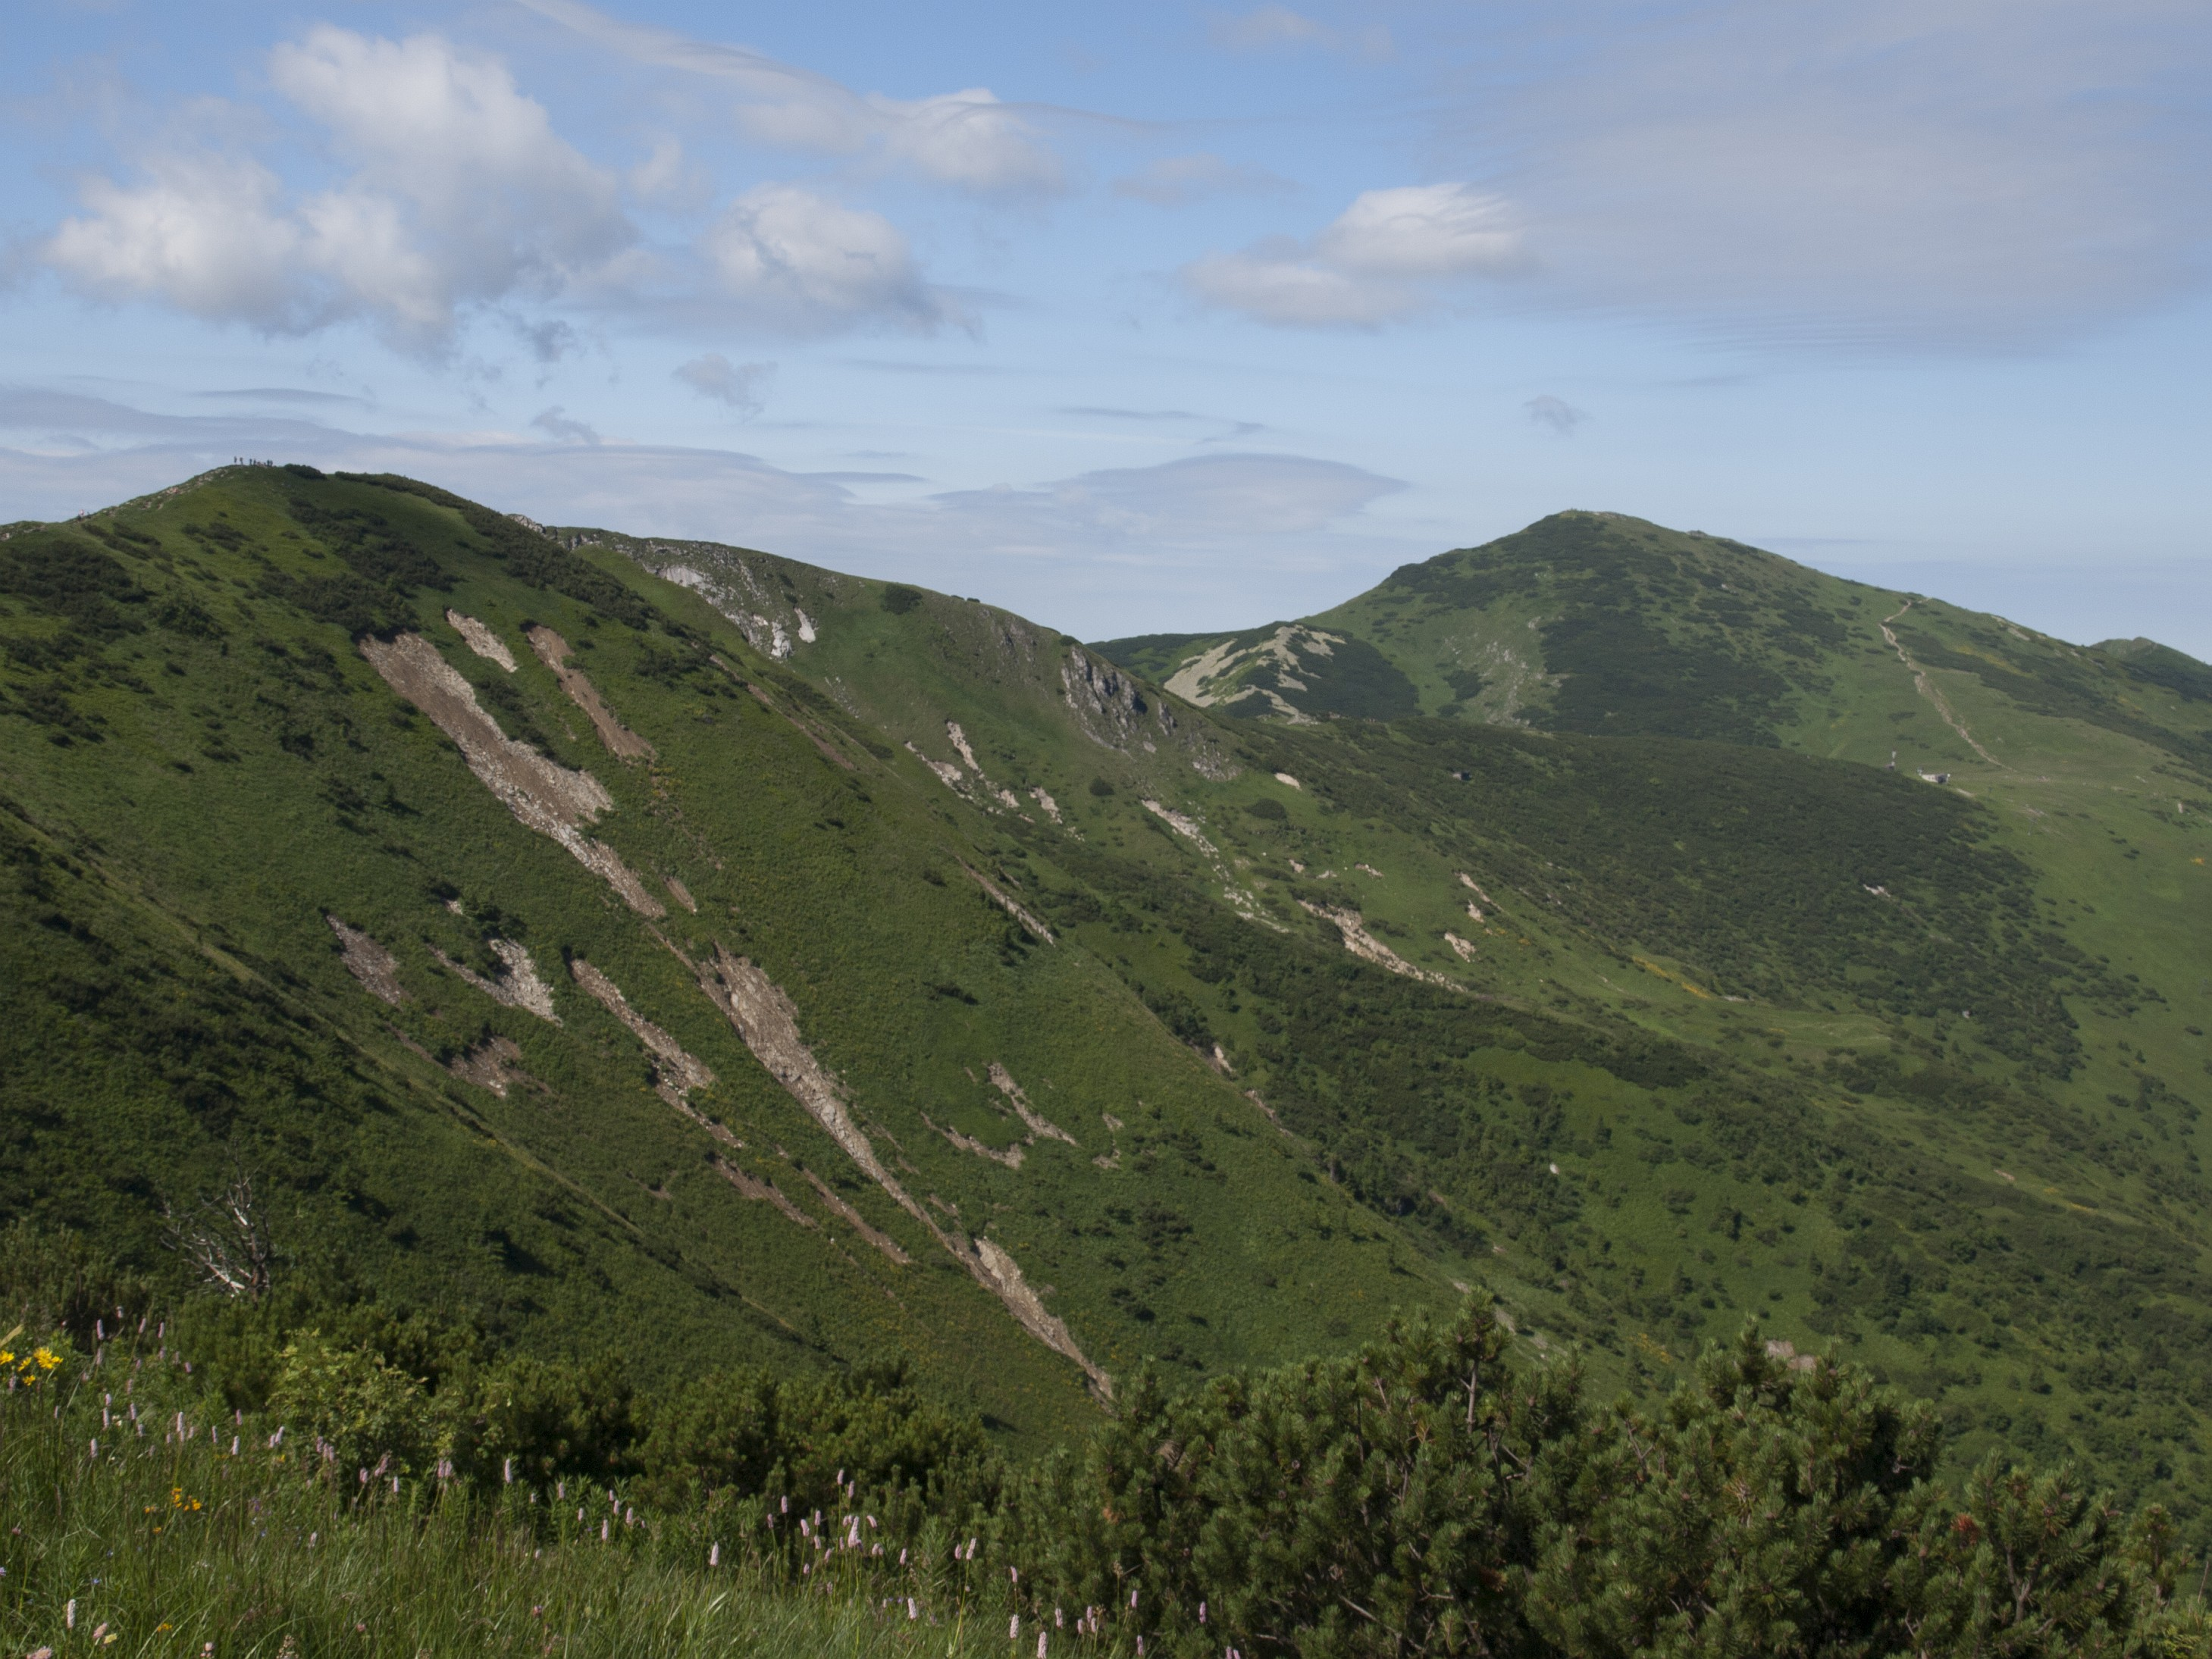
\includegraphics[width=1\linewidth]{obrazky/slope/melke}
	\caption{Mělké translační sesuvy ve zvětralině vzniklé na svazích Chlebu a Hromové v roce 2014 v důsledku intenzivních srážek. Při události došlo k jejich následné transformaci do blokovobahenního proudu, který způsobil velké škody ve Vrátné dolině (Malá Fatra, Slovensko).}
	\label{fig:melke}
\end{figure*}

\subsubsection{Boční rozšiřování}
\emph{Boční rozšiřování} (\textit{lateral spreading}) je rozevírání trhlin pouze horizontálním pohybem v důsledku extenze rigidních (pevných) hornin v nadloží měkkých a plastických hornin. Může se jednat například od pískovce v nadloží jílovců. K bočnímu rozvolňování dochází zpravidla v důsledku pomalé deformace plastického podloží. 

Jedná se o pomalé pohyby (\si{\milli\metre\per\rok}), které ale mohou být extrémně rychlé ve ztekucených zeminách.

\subsubsection{Tečení}
Tečení je svahový pohyb, kdy materiál je ve viskózním stavu. Rychlost tečení je různorodá. Pohybuje se od \si{\centi\metre\per\den} až $>\SI{100}{\kilo\metre\per\hour}$. Výsledný tvar je \emph{proud}. Blokovobahenní proud, mura (debris flow). Hlavní příčinou tečení je nasycení materiálu vodou. Tečením mohou být transportovány i bloky hornin i metrových velikostí. 

\label{blokovo}
Častým typem tečení jsou tzv. \emph{blokovobahenní proudy} (\textit{debris flow}), také nazývané \emph{mury}. Vyskytují se typicky v horském terénu. Jedná se o rychlý pohyb ztekuceného materiálu (bahna a velkých balvanů) ve stržích či údolích prvních řádů, kde se tyto proudy pravidelně opakují. K blokovobahenním proudům dochází zejména po prudkých deštích. Často se vyskytují během povodňových událostí. Prvopočátek blokovobahenního proudu může být v podobě sesuvu vodou saturovaného koluvia. Když tento sesuv narazí na dno strže/údolí dochází ke ztekucení materiálu a vzniku samotného blokovobahenního proudu. Ten má velkou erozní schopnost a díky tomu nabírá další hmotu během svého pohybu.  V případě, že tekoucí materiál neobsahuje velké balvany a skládá se především ze siltu hovoříme o \emph{bahnotoku}. Pro velké bahnotoky a blokovobahenní proudy ze sopečného materiálu se používá termín \emph{lahary}.

\begin{figure}
	\centering
	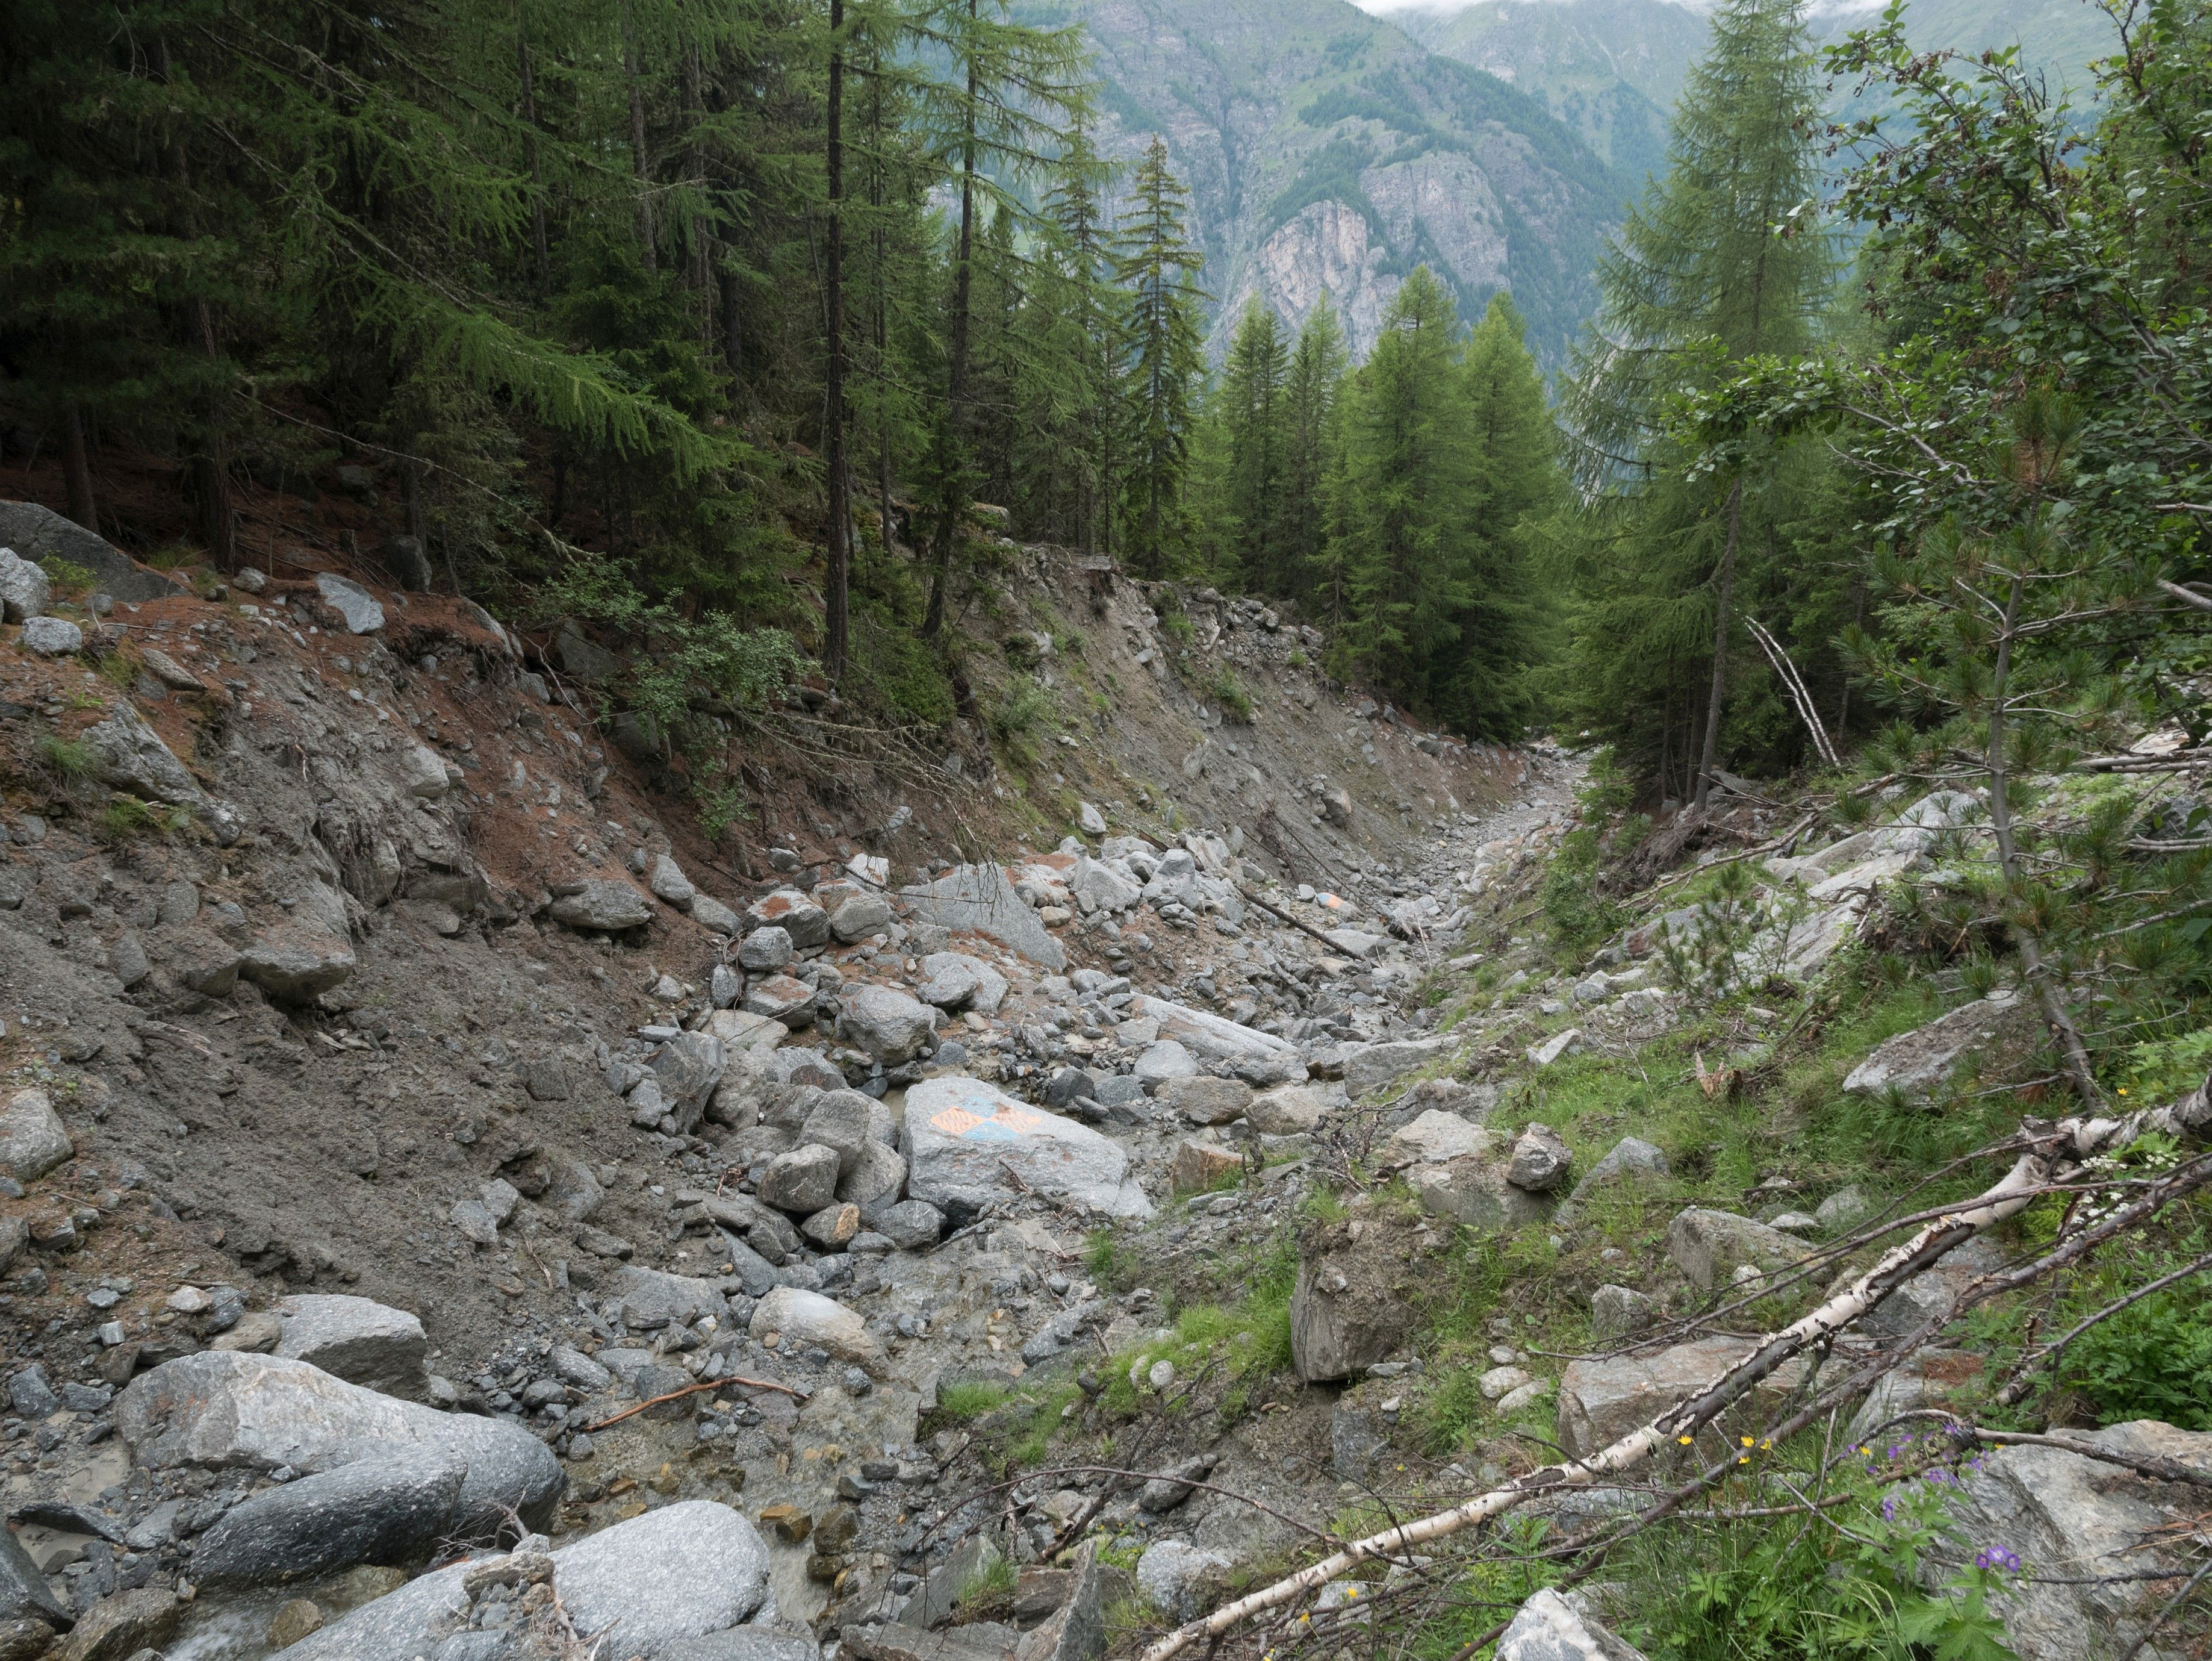
\includegraphics[width=1\linewidth]{obrazky/slope/debris_flow}
	\caption{Dráha blokovobahenních proudů, Švýcarsko.}
	\label{fig:debrisflow}
\end{figure}


\emph{Zemní proud} (\textit{earthflow}) je relativně pomalý proces tečení zemin. Pro zemní proudy jsou typická období klidu (desítky i stovky let) proložená epizodami náhlé aktivity. Jejich rychlost pohybu se pohybuje od metrů za rok až po metry za hodinu. Délka zemních proudů je v řádu desítek metrů až několika kilometrů.

\emph{Skalní laviny} jsou extrémním svahovým procesem. Jejich počátek je zpravidla v podobě velkého skalního sesuvu, který se ale záhy rozpadá a výsledkem je extrémně rychlý proud úlomků hornin. Objem sesunutých hornin bývá $> \SI{1}{\mega\metre\cubed}$ a může dosahovat i desítek \si{\giga\metre\cubed}.
Skalní laviny mají oproti klasickým sesuvům ohromnou mobilitu, tudíž mohou dosáhnout značných vzdáleností od svého počátku (i desítky \si{\kilo\metre}). Rychlost pohybu je v řádu stovek kilometrů za hodinu.

\subsubsection{Svahové deformace}
Termínem \emph{svahové deformace} označujeme extrémně pomalé pohyby (\si{\milli\metre} až \si{\metre\per\rok}) horninových hmot na svahu. Často jsou tyto pomalé pohyby jen přípravnou fází pro jiné, rychlejší svahové procesy. Pomalými pohyby není překročena mez pevnosti hornin, jedná se tak o plastické pohyby, při kterých nevznikají smykové plochy. Podle hloubky do které zasahují pohyby svahové deformace dělíme na:

\begin{itemize}
	\item Povrchové ploužení
	\item Deformace skalních (horských) svahů označované i jako hlubinné ploužení
\end{itemize}

\paragraph{Povrchové ploužení}
Povrchové ploužení je pomalý plastický pohyb zvětralinového pláště (deluvia) a půd na svazích. Projevuje se už na velmi mírných svazích. Hloubkový dosah je v řádu \si{\metre}. K ploužení dochází z důsledku cyklických objemových změn ve zvětralinách v důsledku klimatický vlivů. K expanzi dochází např. při zvlhčení nebo mrznutí, kontrakci pak při vysychání a tání. Dále se uplatňuje růst ledových krystalků \emph{jehlovitého ledu}. Mezi důsledky povrchového ploužení, ale i dobrým identifikačním znakem jsou ohnuté kmeny stromů (tzv. opilý les). Ploužení mů§že způsobovat také  \emph{hákování vrstev}, což je ohnutí vrstev směrem po svahu. 

\emph{Soliflukce} označuje pomalé stékání činné vrstvy permafrostu po zmrzlém podloží, což vede ke vzniku soliflukčních laloků.

\paragraph{Hlubinné ploužení}
Pro hlubinné ploužení se často používá termín \emph{sackung}. Tento proces postihuje velké objemy hornin do značné hloubky (desítky až stovky metrů). Rychlost hlubinného ploužení je velice nízká, což znamená, že se veškeré viditelné formy na svahu vyvíjejí velice pomalu. Sackung se typicky projevuje \emph{zdvojenými hřbety}, různými \emph{stupni na svazích} (Obr \ref{fig:sackung}). Spodní část svahu je často vyboulená. Tento proces vyboulení se označuje jako \emph{bulging}.

\begin{figure}[h]
	\centering
	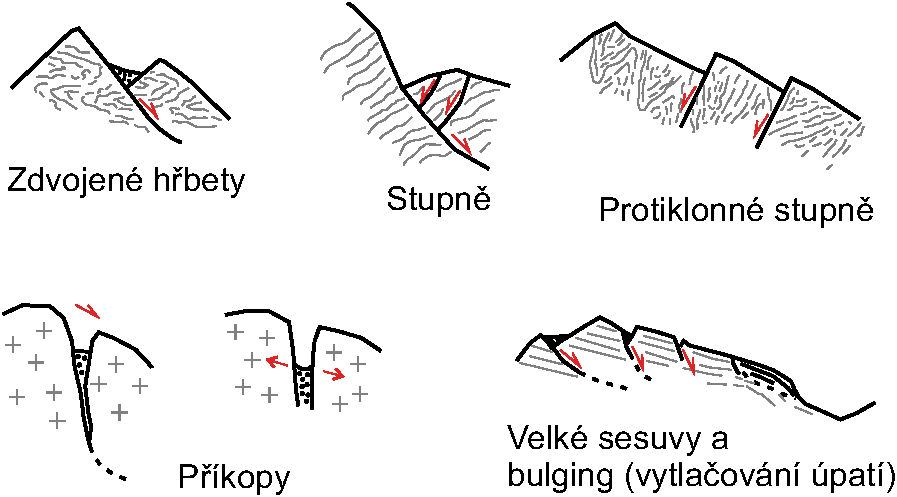
\includegraphics[width=1\linewidth]{obrazky/slope/sackung}
	\caption{Projevy hlubinného ploužení (sackungu) \parencite[podle][]{agliardiStructuralConstraintsDeepseated2001}}
	\label{fig:sackung}
\end{figure}

\subsection{Československá klasifikace svahových pohybů}
Na území ČR je používaná klasifikace svahových pohybů podle Nemčoka, Paška, Rybáře \parencite*{nemcokDeleniSvahovychPohybu1974}. Svahové pohyby dělí na základě mechanismu pohybu a rychlosti pohybu. Tato klasifikace je jednodušší na počet základních typů svahových pohybů, ale v podstatě pokrývá vše co je uvedené v mezinárodní Varnesově klasifikaci. Svahové pohyby dělí do čtyř základních skupin:
\begin{itemize}
	\item ploužení
	\item sesouvání 
	\item stékání
	\item řícení
\end{itemize}

Co je důležité, tak autoři rozlišují \emph{svahový pohyb}, tedy proces a \emph{svahovou deformaci}, což je výsledný tvar. 

\subsubsection{Ploužení}
Do ploužení spadají dlouhodobé pomalé (\si{\milli\metre\per\rok} až \si{\centi\metre\per\rok}). Hranice mezi pohybující se horninovou hmotou a pevným podložím je nezřetelná. V důsledku ploužení může docházet k tzv. hákování vrstev (Obr. \ref{fig:hakovani}). Jedná se ohnutí vrstev po svahu dolů. 
\begin{figure}[h]
	\centering
	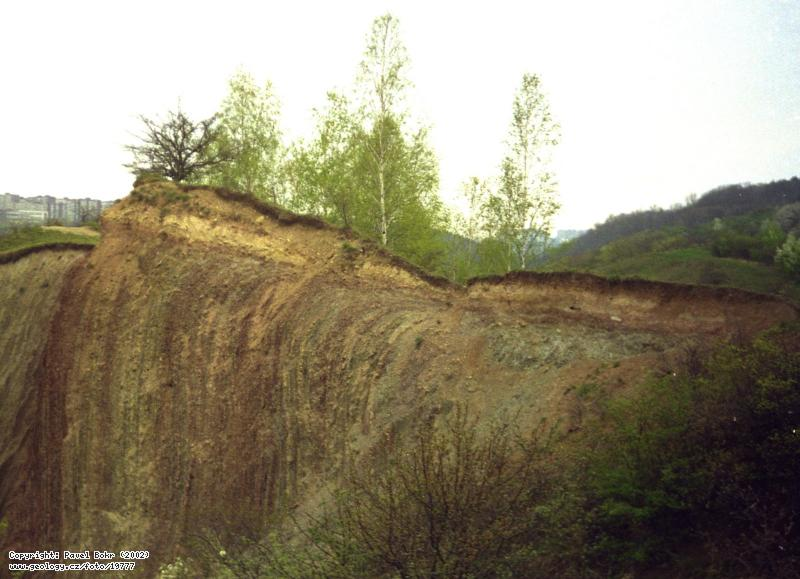
\includegraphics[width=1\linewidth]{obrazky/slope/hakovani}
	\caption{Ukázka hákování vrstev devonských vápenců v Praze-Hlubočepích (Zdroj: BOKR, P. (2002): Foto - Hákování vrstev v Praze - Hlubočepích. In: Fotoarchiv České geologické služby [online databáze]. Praha, Česká geologická služba [cit. 2022-02-15]. Dostupné z URL \url{http://www.geology.cz/foto/19777}}
	\label{fig:hakovani}
\end{figure}

\subsubsection{Sesouvání}
Sesouvání je krátkodobě klouzavý pohyb horninových hmot na svahu podél jedné nebo více průběžných smykových ploch. Jedná se o relativně rychlý pohyb (\si{\centi\metre\per\den} až \si{\metre\per\den}). Výslednou formou sesuvného pohybu je sesuv. Sesuvy dále dělíme podle tvaru smykové plochy (viz výše).

\subsubsection{Tečení}
Stékání je rychlý (\si{\kilo\metre\per\hour}) krátkodobý pohyb horninových hmot ve viskózním stavu. Podstatná část hmot vyteče z odlučného prostoru (jámy) a přemístí se po povrchu terénu na velkou vzdálenost (v ČR i stovky metrů). Stékající hmoty jsou ostře odděleny od neporušeného podloží. Výslednou formou je proud. V konečné fázi vývoje může stékání přecházet do pomalého ploužení. V ČR se vyskytuje nepravidelně a je vázán na extremní srážky spolu s vhodnými geologickými a geomorfologickými podmínkami.

\subsubsection{Řícení}
Krátkodobý (řádově sekundy) rychlý pohyb horninových hmot na strmých svazích, přičemž se postižené hmoty rozvolní a ztrácejí krátkodobě kontakt s podložím. Při pohybu se uplatňuje volný pád. Dříve než hmoty ztratí kontakt s podložím, může docházet k plouživým pohybům. Vzdálenost přemístěných hmot je vzhledem k prostorovým rozměrům zříceného masivu mnohonásobně větší. Tento jev je nejčastěji vyskytuje v oblasti skalních pískovcových měst, u nás např. v oblasti Hřenska, Českého Ráje nebo Broumovska.

% Please add the following required packages to your document preamble:
% \usepackage{booktabs}
% \usepackage{multirow}
% Please add the following required packages to your document preamble:
% \usepackage{booktabs}
% \usepackage{multirow}
\begin{table*}[t]
	\begin{tabularx}{\textwidth}{lp{4.5cm}X}
		\toprule
		& Proces (svahový pohyb)                 & Forma (výsledná svahová deformace)                                                 \\ \midrule
		\multirow{4}{*}{Ploužení}  & Rozvolňování svahů                     & Rozvolnění svahu, roztrhání horských masivů, zdvojené hřbety                       \\
		& Gravitační vrásnění                    & Gravitační vrása, bulging                                                          \\
		& Blokové pohyby                         & Blokové pole                                                                       \\
		& Povrchové ploužení                     & Slézání svahových hlín a suti, hákování vrstev, plošná soliflukce, kamenné ledovce \\ \midrule
		\multirow{3}{*}{Sesouvání} & Sesouvání podél rotační smykové plochy & Rotační sesuv, sesuv podél rotační smykové plochy                                  \\
		& Sesouvání podél rovinné smykové plochy & Planární sesuv, sesuv podél rovinné smykové plochy, skalní sjíždění                \\
		& Sesouvání podél složené smykové plochy & Rotačně planární sesuv, sesuv podél složené smykové plochy, laterální sesuv        \\ \midrule
		Stékání & Stékání svahových uloženin & Zemní proud, bahnitý proud, zemní proud v citlivých jílech, kamenitý, hlinitokamenitý a bahnitý přívalový proud, mura, flowage \\ \midrule
		\multirow{4}{*}{Řícení}    & Sesypávání                             & Drolení, sesyp                                                                     \\
		& Opadávání úlomků                       & Opadový a suťový kužel, osyp, halda, kamenné moře                                  \\
		
		& Odvalové řícení                        & Skalní zřícení, odvalové zřícení                                                   \\
		& Planární řícení                        & Planární skalní zřícení, skalní sesutí \\                                           \bottomrule
	\end{tabularx}
	\caption{Dělení svahových pohybů a svahových deformací dle \textcite{nemcokDeleniSvahovychPohybu1974}.}
	\label{tab:cs_klasifikace}
\end{table*}



\subsection{Další klasifikace svahových pohybů a jejich výsledných forem}
Výše uvedené klasifikace jsou založené jen na několika málo kritériích (mechanismus pohybu, rychlost, materiál). Pro zjednodušení budu v této pasáži budu používat pojem sesuv ve volnějším pojetí jako zastřešující termín dalších výsledných forem (např. zemního proudu).

Z hlediska stáří rozlišujeme sesuvy recentní (současné), historické a fosilní.

Podle aktivity rozlišujeme sesuvy na \emph{aktivní} (živý), kdy právě dochází k pohybu. V případě, že na přechodnou dobu ustaly podmínky, které způsobovaly pohyb, jedná se o sesuv \emph{dočasně uklidněný}. Pokud ani změna podmínek nemůže způsobit reaktivaci sesuvu, jedná se o sesuv stabilizovaný.

věk: recentní (současný, čerstvý), fosilní (starý)
stupeň aktivity: aktivní (živý), dočasně uklidněný, stabilizovaný (zastavený)
geneze: přirozený (samovolný), uměle vyvolaný (antropogenní)
vývojové stadium: iniciální (počáteční), rozvinutý (pokročilý), finální (závěrečné)
opakovatelnost: jednorázový, periodický
tvar půdorysu: proudový, frontální, plošný, nepravidelný
zřetelnost morfologické formy: zřetelná svahová deformace, zastřená svahová deformace, pohřbená svahová deformace
pozice vůči dalším svahovým deformacím: samostatná svahová deformace, složená svahová deformace, součást složené svahové deformace


\section{Geomorfologické důsledky svahových procesů}
Propojení vodních toků a svahů je důležité z chodu sedimentů. 


Způsob jakým jsou sesuvy a další gravitační procesy propojené s vodními toky lze rozdělit do pěti skupin \parencite{korupGeomorphicImprintLandslides2005}. 

\begin{enumerate}
	\item Plošné - rozsáhlé rozsáhlých svahových deformací, které překračují jednotlivá rozvodí
	\item Liniové -- sesuv ve svém pohybu pokračuje v údolí ve vodním toku. Dojde například k tranformaci sesuvu na blokovobahenní proud apod
	\item Bodové -- akumulační oblast sesuvu zasahuje do vodního toku.
	\item Nepřímé -- Nepřímé působení je v případě sesunutí do vodní nádrže (přírodní či umělé).
	\item Žádné -- nedochází k interakci mezi sesuvem a vodním tokem (akumulace nezasahuje na dno údolí)
\end{enumerate}

\begin{figure}[h]
	\centering
	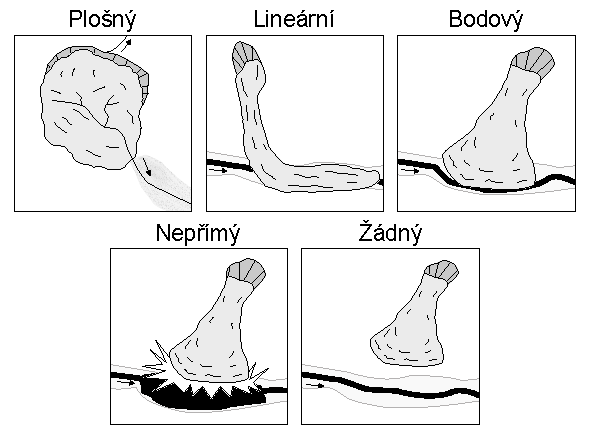
\includegraphics[width=1\linewidth]{obrazky/slope/korup_toky}
	\caption{Možné interakce mezi vodním tokem a sesuvem (upraveno podle \textcite{korupGeomorphicImprintLandslides2005})}
	\label{fig:koruptoky}
\end{figure}



\section{Eroze na svazích}

\subsection{Difuzní procesy}
Difuzní procesy jsou charakteristické tím, že se na transportu sedimentů nepodílí soustředěný tok vody, větru či ledu. Tyto procesy zahlazují nerovnosti na svahu a postupně snižují vertikální členitost reliéfu. 

\emph{Bombardování vodními kapkami} se uplatňuje zejména tam, kde \emph{vegetační kryt je velice řídký či zcela chybí} (pouště, badlandy). Vodní kapka, která dopadá na ukloněný povrch vymrští částečky, které letí proti a po svahu. Ty, které jsou odmrštěny proti svahu mají kratší trajektorii, než ty, které letí po svahu dolů. Tímto způsobem se tak materiál postupně přesouvá směrem po svahu. samozřejmě čím větší je sklon, tím delší je transport po svahu dolů.
%\todo[inline]{přidat obr. kapky}

Významnějším procesem je \emph{plošný (ronový) splach}. Jako \emph{ron} označujeme nesoustředěný odtok vody po povrchu. Největší účinky má plošný splach opět na svazích, které nejsou pokryté vegetací. K tomuto \emph{povrchovému odtoku} dochází při překročení infiltrační kapacity půdy nebo jejímu nasycení vodou. Se zvětšujícím se sklonem a narůstajícím množstvím vody se laminární proudění mění na turbulentní. To způsobuje soustředění odtoku a začátek hloubkové eroze, což v důsledku vede ke vzniku stružek a následně strží.

Do difuzních procesů se řadí i povrchové ploužení, ale o něm byla řeč již výše.

\subsection{Liniová eroze}
Soustředěním povrchového odtoku a vznikem turbulentního proudění dochází k intenzivní výmolné činnosti v místech soustředění. Iniciálním stádiem liniové eroze je \emph{stružková eroze}. \emph{Stružky} jsou mělké erozní rýhy, které jsou občasně protékané vodou. Většinou se jedná o systém paralelních pravidelně uspořádaných rýh. Vznikají v důsledku silných srážek nebo rychlého tání sněhu na vegetací nekrytých površích. 

Rozvojem stružek, jejich prohlubováním a prodlužováním do podoby, kdy jsou již trvalou součástí krajiny (např. jsou tak velké, že je nelze zaorat) vznikají \emph{strže}. Hovoříme pak o \emph{stržové erozi}. Strže mohou být občasně, ale i trvale protékané vodním tokem. 

\emph{Badland} je erozí zcela přemodelovaná plocha. Jedná se o hustou síť strží a stružek. Půda prakticky absentuje a vegetace je velice sporá. Badlandy často vznikají antropogenní příčinou. 

Intenzivní a člověkem urychlená eroze ze svahů (např. odlesněním, špatným hospodařením na polích) není problematická jen z důvodu ztráty půdy z daného místa a zmenšení obdělávatelných ploch. Materiál, který je odnesen se dostává do vodních toků, což snižuje kvalitu vody ale také materiál někde sedimentuje a to může způsobovat další problémy. 

\subsection{Sufoze}
\emph{Sufoze} je proces při kterém dochází k odnosu částic pod povrchem. Voda se dostává do podloží a následně soustavou drobných tunelů (\textit{pipes}) odtéká a odplavuje materiál. Sufoze nemusí být na povrchu patrná. Postupným zvětšováním tunelů ale následně může docházet ke kolapsům povrchů a vznikají \enquote{závrty}. V některých místech mohou tunely ústit na povrch a vytvářejí tak otevřené kanály, kde se na úpatí ukládá vyplavený materiál. Sufoze tak může předcházet následnému rozvoji strží. 

%\newpage
%\onecolumn
%\begin{boxotazky}{Kontrolní a klíčové otázky, na které bychom měli znát odpověď}
%	\begin{itemize}
%		\item Co ovlivňuje stabilitu  svahu?
%		\item Jaké síly působí na svah? Jak jejich rozložení ovlivňuje sklon svahu?
%		\item Jaké základní svahové procesy známe?
%		\item 
%	\end{itemize}
%\end{boxotazky}
%
%\begin{boxslovnik}{Další klíčové pojmy k zapamatování}
%	aaa & adfasd \\
%	
%\end{boxslovnik}
%\twocolumn